\chapter{Aspectos numéricos}
Nesta seção serão analisados os algoritmos principais do nosso projeto, entre eles: solução numérica da EDO (\ref{ModeloDeterministicoEDO}), solução analítica da EDO (\ref{ModeloDeterministicoEDO}), solução numérica da EDE(\ref{Cubo}), as distribuições uniforme, Gaussiana, exponencial e por fim o movimento Browniano. Para cada um desses algoritmos será elaborado um gráfico com o tempo de execução em função da entrada exibindo o crescimento do tempo de execução da função e a quantidade de memória gasta por cada algoritmo. Vamos definir que complexidade espacial é a quantidade de memória alocada por uma função

\section{Distribuição uniforme}
O código (\ref{d_Uniforme}) apresenta uma simples chamada a função frand() definida como pré processor (por razões de eficiência) dentro de um laço. A complexidade espacial é de $O(n)$ pois a função aloca \textit{n} doubles onde \textit{n} é o numero de pontos. O tempo de execução em função da entrada pode ser visto na figura (\ref{TempExecUniforme}).
\begin{figure}[!htb]
\centering
\begin{minipage}[b]{0.45\linewidth}
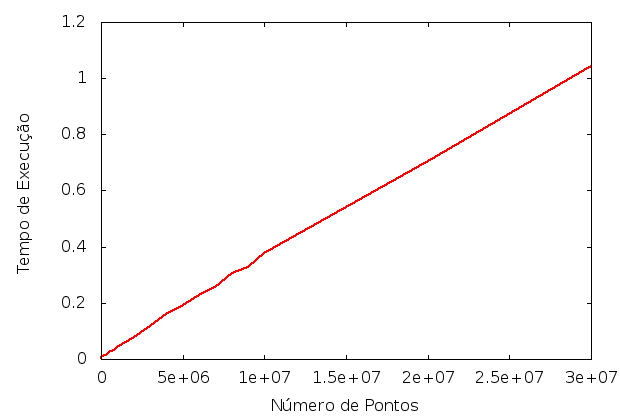
\includegraphics[width=\linewidth]{./img/AspectosNumericos/UniComplexidade.png}
\caption{Distribuição uniforme - tempo de execução}
\label{TempExecUniforme}
\end{minipage} \hfill
\end{figure}

\section{Distribuição Gaussiana}
O código (\ref{d_Gaussiana}) apresenta complexidade espacial é de O(3n) pois aloca 3 arrays de doubles 2 para distribuições uniformes e 1 para o retorno do método. O tempo de execução em função da entrada pode ser visto na figura (\ref{TempExecGau}).
\begin{figure}[!htb]
\centering
\begin{minipage}[b]{0.45\linewidth}
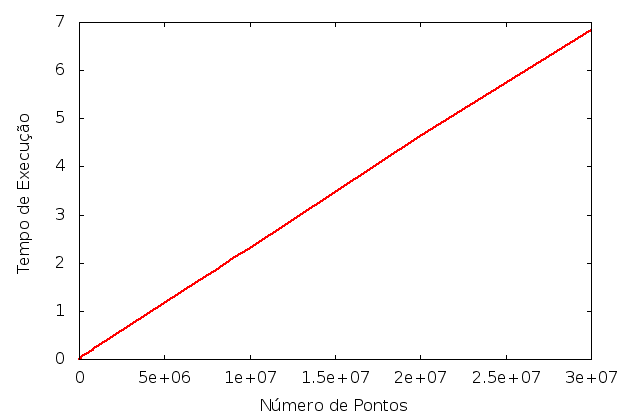
\includegraphics[width=\linewidth]{./img/AspectosNumericos/GauComplexidade.png}
\caption{Distribuição  Gaussiana- tempo de execução}
\label{TempExecGau}
\end{minipage} \hfill
\end{figure}

\section{Distribuição Exponencial}
O código (\ref{d_Exponencial}) apresenta a complexidade espacial é de O(2n) pois aloca 2 arrays de doubles 1 para distribuição uniforme e 1 para o retorno do método. O tempo de execução em função da entrada pode ser visto na figura (\ref{TempExecExp}).
\begin{figure}[!htb]
\centering
\begin{minipage}[b]{0.45\linewidth}
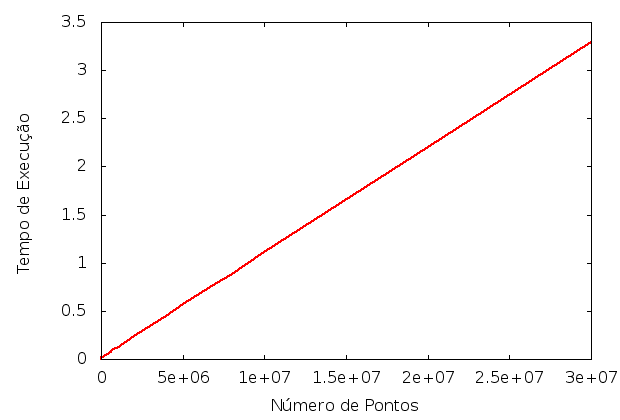
\includegraphics[width=\linewidth]{./img/AspectosNumericos/ExponencialComplexidade.png}
\caption{Distribuição exponencial - tempo de execução}
\label{TempExecExp}
\end{minipage} \hfill
\end{figure}

\section{Movimento Browniano}
O código (\ref{movimentoBrownianoFONTE}) apresenta a complexidade espacial é de $O(n)$ pois aloca um vetor de doubles para retornar o movimento discretizado. O tempo de execução em função da entrada pode ser visto na figura (\ref{movBrownianoTempExec}).
\begin{figure}[!htb]
\centering
\begin{minipage}[b]{0.45\linewidth}
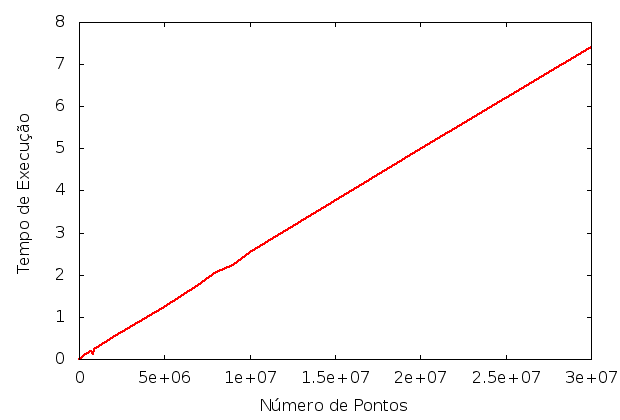
\includegraphics[width=\linewidth]{./img/AspectosNumericos/MBComplexidade.png}
\caption{Movimento Browniano- tempo de execução}
\label{movBrownianoTempExec}
\end{minipage} \hfill
\end{figure}

\section{Análise solução numérica EDO}
Ao analisar o código (\ref{EDOFONTE}) a complexidade espacial (quantidade de memória gasta) é dada como: 1 array de doubles cujo tamanho é igual ao número de pontos (n) acrescidos de dois doubles por iterada cujo escopo é o laço, logo podemos afirmar que a complexidade espacial é $O(n) * 8bytes$ (tamanho de um double em C). O tempo de execução em função da entrada pode ser visto na figura (\ref{tmpExecEuler}).
\begin{figure}[!htb]
\centering
\begin{minipage}[b]{0.45\linewidth}
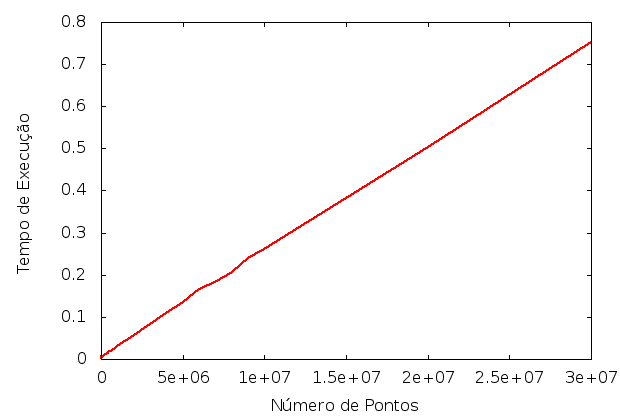
\includegraphics[width=\linewidth]{./img/AspectosNumericos/EulerComplexidade.png}
\caption{Solução númerica EDO - tempo de execução}
\label{tmpExecEuler}
\end{minipage} \hfill
\end{figure}

\section{Análise solução analítica da EDO}
Ao analisar o código (\ref{EDOFONTE}, podemos afirmar que, em termos de memória alocada a função apresenta alocação de 2 vetores de double proporcionais ao número de pontos logo a complexidade em termos de espaço é de $O(2n) * 8bytes$ (tamanho de um double em C). O tempo de execução em função da entrada pode ser visto na figura (\ref{tmpExecAnalitica}).
\begin{figure}[!htb]
\centering
\begin{minipage}[b]{0.45\linewidth}
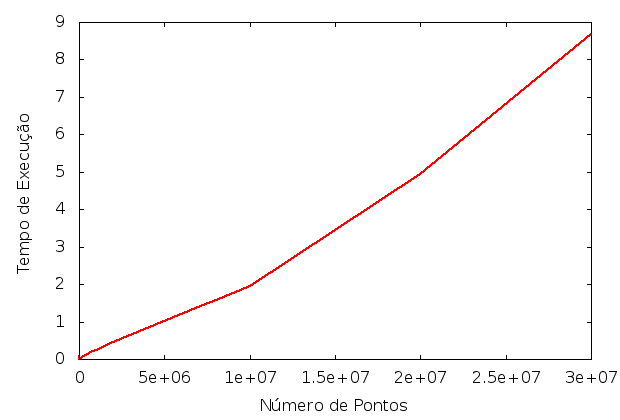
\includegraphics[width=\linewidth]{./img/AspectosNumericos/SolExacComplexidade.png}
\caption{Solução analítica EDO - tempo de execução}
\label{tmpExecAnalitica}
\end{minipage} \hfill
\end{figure}

\section{Análise solução numérica EDE Langevin}
O código (\ref{EDEFONTE}) a complexidade espacial é de O(n) dado que a função aloca n doubles para utilizar como retorno, a EDE com ruído recursivo tem a mesma complexidade porém apresenta mais multiplicações. O tempo de execução em função da entrada pode ser visto na figura (\ref{tmpExecNumericaEDE}).
\begin{figure}[!htb]
\centering
\begin{minipage}[b]{0.45\linewidth}
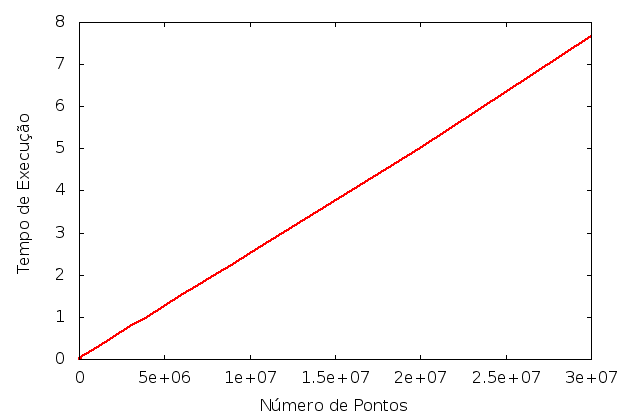
\includegraphics[width=\linewidth]{./img/AspectosNumericos/EulerMaruyamaComplexidade.png}
\caption{Solução numérica EDE - tempo de execução}
\label{tmpExecNumericaEDE}
\end{minipage} \hfill
\end{figure}


